\documentclass[12pt]{article}
\usepackage[left=.5in, right=.5in, top=.5in, bottom=.5in]{geometry}
\usepackage[parfill]{parskip}
\usepackage{amsmath, amssymb, enumitem, graphicx}
\pagenumbering{gobble}
\setlength\parindent{0pt}

\begin{document}

\begin{center}
{\Large CSC413H1 - Assignment 3}
\end{center}

\textbf{1.1.1:} I expect the optimal learning rate to increase since the noise of the minibatch gradient would decrease. If $B$ is initially small, this increase in the rate would be larger than if $B$ is initially large.

\textbf{1.1.2:}
\begin{enumerate}[label=(\alph*)]
    \item Point C, since for batch sizes larger than C's, increasing the batch size requires more compute but does not reduce the training time by much, while for batch sizes smaller than C's, increasing the batch size can reduce the training time with a small change in compute.
    \item Point A: noise dominated, seek parallel compute. Point B: curvature dominated, use higher order optimizers.
\end{enumerate}

\textbf{1.2:} Option C, since figure 2 shows that the compute-efficient training phase stops short of convergence even with more steps. In addition, figure 3, which is plotted using the critical batch sizes, indicates that increasing the model size is more helpful than changing the batch size.

\textbf{Scaled Dot Product Attention:}
\begin{enumerate}
    \item See the attached code.
    \item See the attached code.
    \item Since transformers process words in parallel, positional encoding allows the models to include information about the word order, which is important to semantics. Sine and cosine encoding are advantageous since they require fewer dimensions compared to one hot encoding, especially for longer sequences, and this makes them more efficient.
    \item The lowest validation losses are:
    \begin{itemize}
        \item 0.9034 for the small dataset with a hidden size of 32;
        \item 0.6448 for the large dataset with a hidden size of 32;
        \item 0.4199 for the small dataset with a hidden size of 64;
        \item 0.2936 for the large dataset with a hidden size of 64.
    \end{itemize} The plots are shown below:
    \begin{center}
        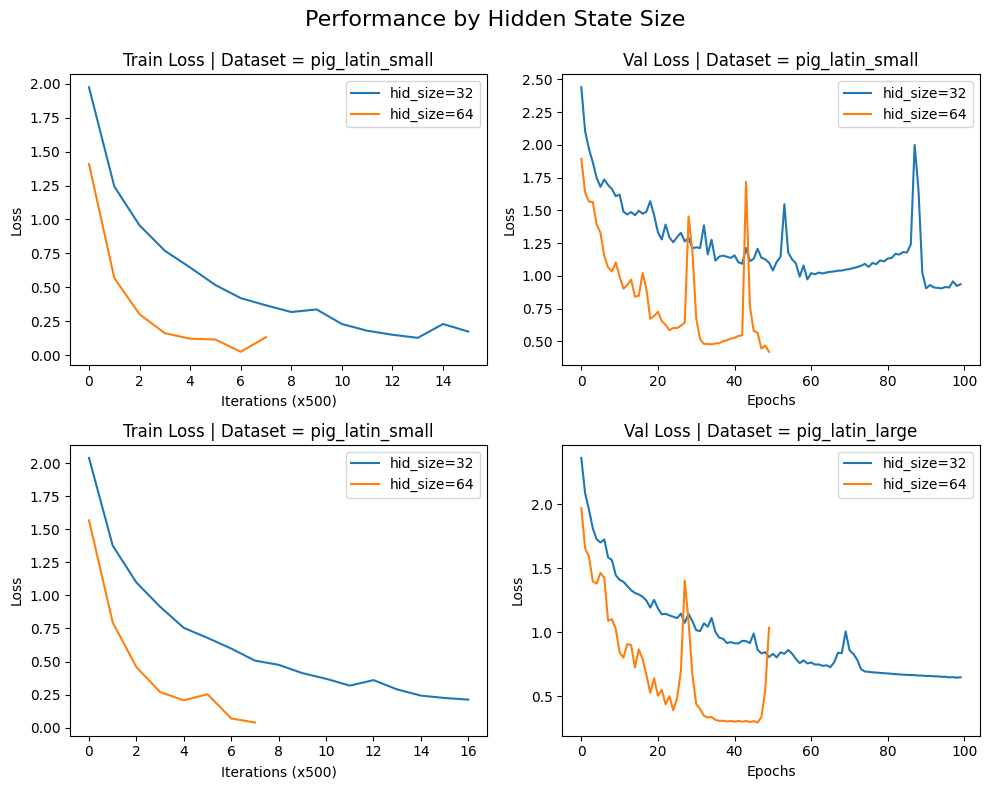
\includegraphics[scale=.6]{2.1.4-1.png}
        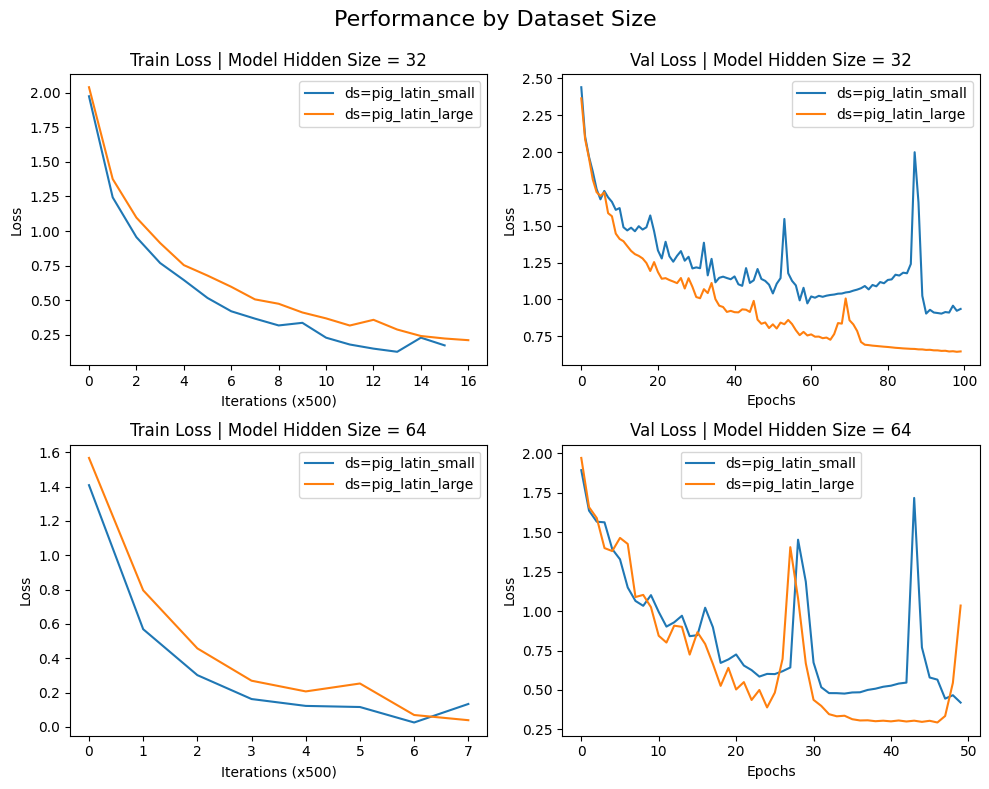
\includegraphics[scale=.6]{2.1.4-2.png}
    \end{center} Thus, increasing the model capacity and increasing the dataset size both decrease the lowest validation loss, meaning that they improve the generalization of the model. The first four plots show that increasing the capacity also helps the model to converge faster. These results are not surprising since a larger model can be more powerful and capable of learning the patterns in the data, while a larger dataset allows the model to learn a more general representation of the data.
\end{enumerate}

\textbf{Decoder Only NMT:}
\begin{enumerate}
    \item See the attached code.
    \item See the attached code.
    \item Pros: The decoder-only model has a simpler architecture since it does not need to encode a hidden state of the input, which makes training easier. Cons: In general, decoder-only models are limited to autoregressive textual tasks, whereas encoder-decoder models can also be used for other tasks such as multimodal learning.
    
    The decoder-only model performs better than the encoder-decoder model since their lowest validation losses are 0.2660 and 0.2936 respectively, while their test translation outputs are the same.
\end{enumerate}

\textbf{Scaling Law and IsoFLOP Profiles:}
\begin{enumerate}
    \item The polynomial approximation plot  is shown below:
    \begin{center}
        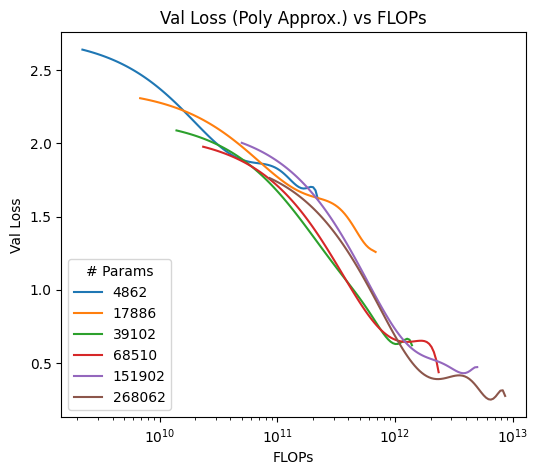
\includegraphics[width=.5\linewidth]{2.3.1.png}
    \end{center}
        As FLOPs increase, the validation loss generally decreases for all six models, with the change in loss being smoother for smaller FLOPs and more stochastic for larger FLOPs. Consistent with figure 3 in 1.2, the plot shows that a larger model generally has a smaller loss.
    \item The plot is shown below:
    \begin{center}
        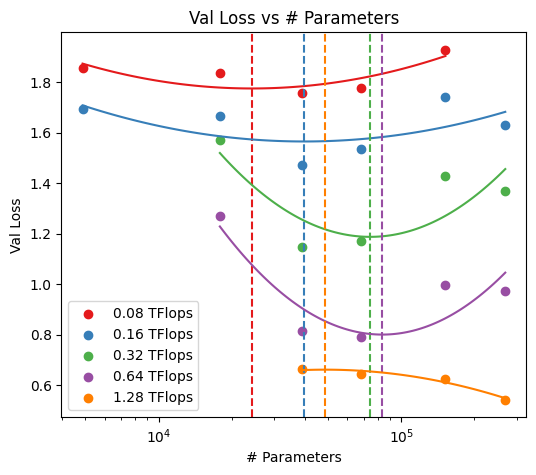
\includegraphics[width=.5\linewidth]{2.3.2-2.png}
    \end{center}
    \item The plot is shown below:
    \begin{center}
        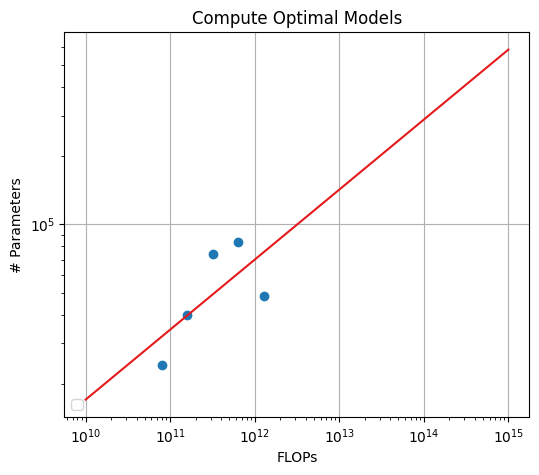
\includegraphics[width=.5\linewidth]{2.3.3-2.png}
    \end{center} Based on the plot and its equation $\log_{10}(y) = 0.3071\log_{10}(x) + 1.1593$, the optimal number of parameters for a compute budget of $1e15$ is approximately $5.837e5$.
    \item The training setup in 2.2.3 is not compute optimal, since the training epochs with FLOPs close to the target FLOPs (specifically epochs 0, 1, 3, 6, and 14) have fewer tokens compared to the optimal numbers of tokens for those FLOPs in the plot. To change it, we should increase the number of tokens by increasing the batch size or increasing the sequence length of \texttt{SOS\_src\_EOP\_tgt}. In addition, the setup has 268062 parameters, which is less than the optimal number of parameters for all target FLOPs, so we should increase the number of parameters as well.
    \begin{center}
        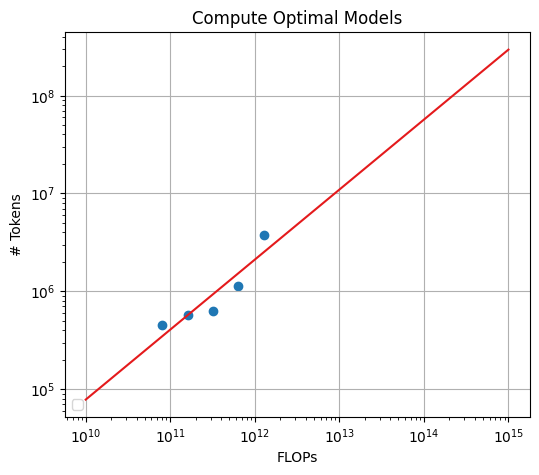
\includegraphics[scale=.6]{2.3.4.png}
    \end{center}
\end{enumerate}

\textbf{BERT:}
\begin{enumerate}
    \item See the attached code.
    \addtocounter{enumi}{1}
    \item The train time is reduced (1 second vs. 6 seconds), likely because there is no gradient computation needed for the frozen layers. The validation accuracy is lower (0.74 vs. 0.92), likely because the frozen layers cannot learn new information about the inputs that would help the classifier be more accurate for this specific task.
    \item The validation accuracy is lower (0.72 vs. 0.92). This is likely because the BERTweet dataset has less math-related data than the MathBERT dataset, and thus pre-training on BERTweet is less effective for math-related tasks than pre-training on MathBERT.
\end{enumerate}

\textbf{CLIP:} The caption is "orange fish". The process was easy since the main visible features of the target image were "orange" and "fish".

\end{document}